
\chapter{Cache evaluation analysis}

\section{Payloads}

\subsection{Zephyr based matrix-multiplication}

% TODO: is zephyr even imporant here? idk
Matrix multiplication is a fundamental operation in many scientific and engineering applications, including high-performance computing (e.g., finite element methods), machine
learning (e.g., linear algebra), and edge computing (e.g., DSP, edge-AI, cryptography), among others. This section discusses the implementation and of various cache multiplication algorithms,
taking into the account cache usage in each of them.

The algorithms have been implemented using the Zephyr RTOS as the execution platform. This particular RTOS has been chosen due to its support for a wide range of hardware boards,
its user-friendly build system (\texttt{CMake} alongside the \texttt{west} helper), its use of the C programming language, and its robust real-time capabilities.
Moreover, Zephyr is a collaborative project with the Linux Foundation and is the fastest-growing real-time operating system \cite{zephyrlotsofcommits}. It has commercial support
from major vendors in the embedded and edge computing sectors, such as Nordic Semiconductors, NXP, STMicroelectronics, Microchip, and many others \cite{aboutzephyr}. Additionally,
it is backed by major companies in the technology sector, including, among others, Google, Meta, Qualcomm and Intel \cite{zephyrmetagoogle, zephyrmembers}.

\noindent This payload will be used for testing \textit{different software configurations}, while the simulated \textit{hardware remains unchanged}.

\subsubsection*{Naive approach} \label{sec:mmnaive}
The naive approach to matrix multiplication involves three nested loops iterating over the rows and columns of the matrices. This method, is called naive, as it is simple, but not cache-friendly
due to its poor data locality.

\begin{center}
	\centering
	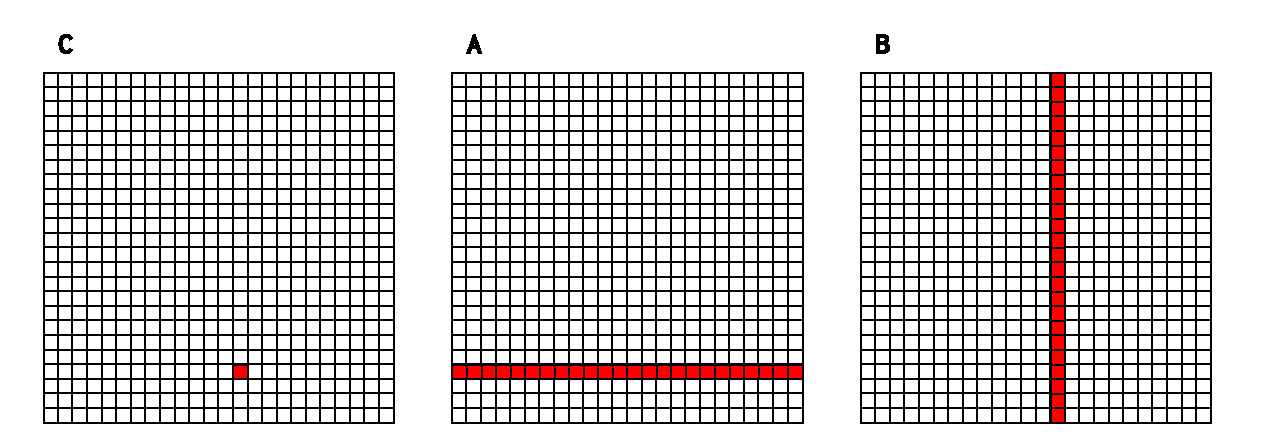
\includegraphics[width=0.75\textwidth]{figures/05-analysis/mm_naive.pdf}
	\captionof{figure}{Visual representation of the multiplication using the naive approach}
	\label{fig:mm_naive}
\end{center}

The naive approach involves three nested loops, iterating over the rows columns of the matrices:

\begin{center}
\centering
\begin{minipage}{\linewidth}
\begin{lstlisting}[
	style=lstC,
    caption={Naive matrix multiplication implemented in C programming language}
    ]
for (i = 0; i < SIZE; i++) {
	for (j = 0; j < SIZE; j++) {
		for (k = 0; k < SIZE; k++) {
			c[i * SIZE + j] += a[i * SIZE + k] * b[k * SIZE + j];
		}
	}
}
\end{lstlisting}
\end{minipage}
\end{center}

\noindent If the matrices are represented as a 1D array in memory, the naive approach to matrix multiplication results in poor cache performance due to suboptimal data locality.
The naive algorithm frequently jumps between distant memory locations, leading to cache misses.

\subsubsection*{Block based approach} \label{sec:mmblock}
The block-based approach improves cache performance by dividing the matrices into smaller sub-matrices (blocks) that fit into the cache.

\begin{center}
	\centering
	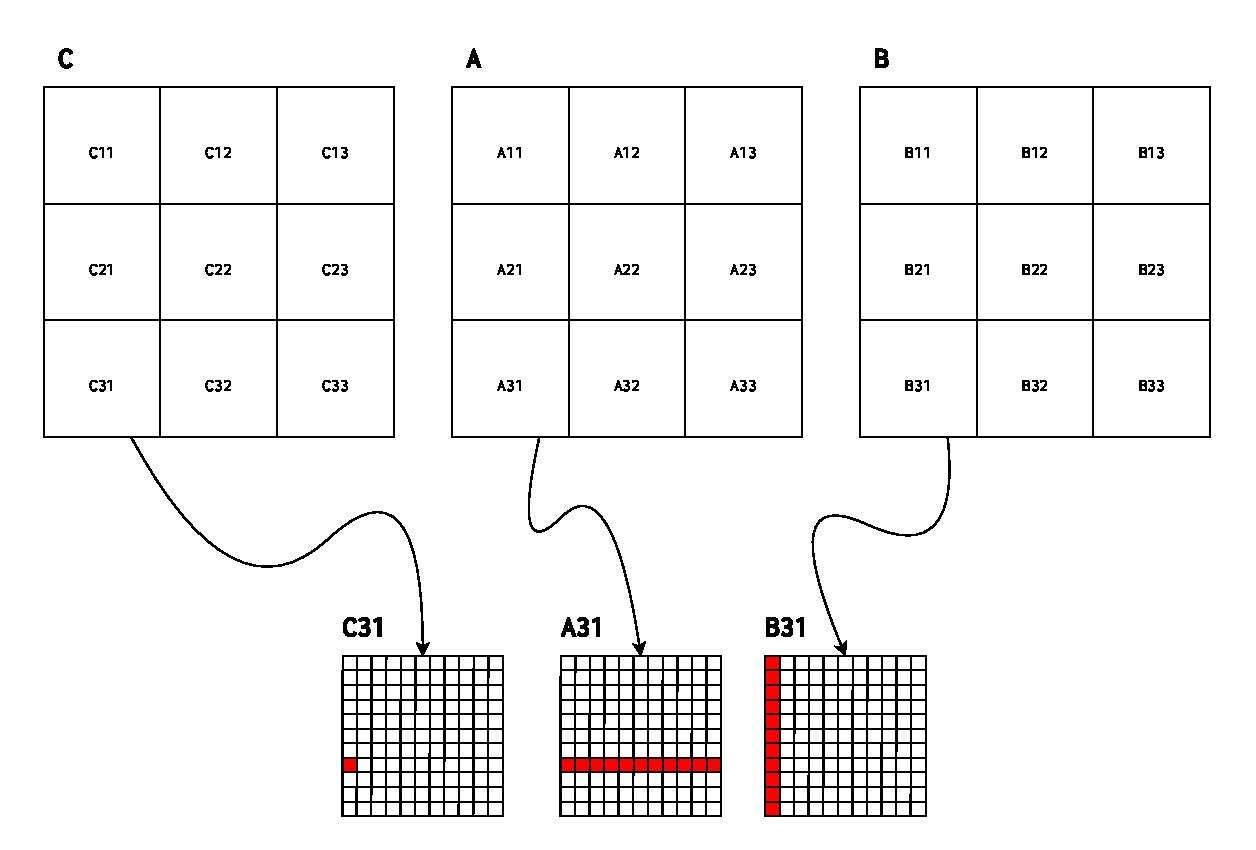
\includegraphics[width=0.75\textwidth]{figures/05-analysis/mm_block.pdf}
	\captionof{figure}{Visual representation of the multiplication using the block based approach}
	\label{fig:mm_block}
\end{center}

\noindent By dividing the large matrix into smaller matrices, data locality is significantly improved, reducing the number of cache misses. This method is particularly effective for
large matrices, where the naive approach would otherwise result in frequent cache evictions. The larger blocks (A11, A12, B11, B12, etc.) are then multiplied and added together.
Selecting the optimal block size is a trade-off. The block size should be small enough to allow the data to fit into the cache but as large as possible to minimize runtime
overhead. Decreasing the block size results in increased runtime overhead because more instructions need to be executed.

\noindent The block-based algorithm has been implemented as follows:
\begin{center}
\centering
\begin{minipage}{\linewidth}
\begin{lstlisting}[
	style=lstC,
    caption={Block based matrix multiplication in C programming language}
    ]
const int B = BLOCK_SIZE;
for (i = 0; i < SIZE; i += B) {
	for (j = 0; j < SIZE; j += B) {
		for (k = 0; k < SIZE; k += B) {
			/* B x B mini matrix multiplications */
			for (i1 = i; i1 < i + B && i1 < SIZE; i1++) {
				for (j1 = j; j1 < j + B && j1 < SIZE; j1++) {
					for (k1 = k; k1 < k + B && k1 < SIZE; k1++) {
						c[i1 * SIZE + j1] += a[i1 * SIZE + k1] * b[k1 * SIZE + j1];
					}
				}
			}
		}
	}
}
\end{lstlisting}
\end{minipage}
\end{center}

\subsection{Linux kernel}
% TODO: this section is a biiit short
The Linux kernel is a core component of many devices, ranging from relatively small microcontrollers, to desktop computers and even HPC clusters.
It has been selected as a payload due to its relatively lengthy and memory-access-intensive boot process, such as during the unpacking of initramfs. This process is
characterized by a mix of sequential and random memory access patterns, providing a good benchmark for testing various cache configurations.

\noindent This payload will be used for testing \textit{different hardware configurations}, while the \textit{software remains unchanged}.

\section{Cache model verification}

To validate the model, it was tested against two independent data sources. The first validation was performed using the QEMU TCG Cache Modeling plugin as a reference, and the
second test was conducted by using a hardware device with built in hardware performance counters. The data input for the cache model implemented in this work was generated using
the Renode framework. This constrains the hardware choice to platforms that are compatible with both QEMU and Renode and are readily available for purchase on the market.

The RISC-V-based SiFive HiFive1 Rev B (\texttt{fu310} SoC with one \texttt{e31} RV32IMAC core) platform has been selected. This platform meets the necessary requirements for
compatibility with both QEMU and Renode, provides extensive documentation including cache parameters, and features built-in hardware performance counters.
The cache configuration for the \texttt{e31} core includes a 16 KiB 2-way set-associative instruction cache with a 32-byte block line size with \textit{random} eviction policy and
no data cache \cite{fe310docs}.

\subsection{Generating cache statistics} \label{sec:gencachestats}

The payload against which the verification was performed is the Zephyr RTOS-based matrix multiplication algorithm (naive approach). Due to the
platform's limited RAM size, the benchmark sample had to be limited to a matrix of size 16 by 16\footnote{Matrices of size $32^2$ resulted in a stack crash (manifesting itself in
a \textit{Load access fault} exception), while sizes $64^2$ and above resulted in a linker failure due to overflowing memory regions.}. The cache usage statistics are gathered
starting from the platform reset, and ended at the \texttt{finished()} symbol entry point, a helper function that marks the end of the matrix multiplication algorithm.\label{snip:measurement_window}

\subsubsection{Novel cache model \& Renode ExecutionTracer} % XXX: replace "novel"
In order to easily gather the cache statistics from the novel cache model, using the Renode framework as a trace generation backend, an \textbf{"Automated Renode Cache Test Executor"} % XXX: replace "novel"
toolset was prepared. Is a wrapper, written in bash, that configures, and pipelines the execution of both Renode and Cache model: % XXX: toolset?


\begin{center}
\centering
\begin{minipage}{\linewidth}
\begin{lstlisting}[
    language=Bash,
    caption={Automated Renode Cache Test Executor}
    ]
#!/usr/bin/env bash

DIRECTORY=$1
PRESET=$2
TRACE_DIR="$(realpath traces)"
RESULT_DIR="$(realpath results)"
RENODE_LOG="RENODE_LOG"

for ELF_FILE in "$DIRECTORY"/*.elf; do
	if [ -f "$ELF_FILE" ]; then
		ELF_PATH="$(realpath $ELF_FILE)"
		ELF_FNAME=$(basename -- "$ELF_FILE" .elf)
		TRACE_PATH="$TRACE_DIR/$ELF_FNAME.log"
		RESULT_PATH="$RESULT_DIR/$ELF_FNAME.txt"

		echo "[$(date +%H:%M:%S)] Genrating traces using Renode for $ELF_FNAME" tee -a "$RENODE_LOG"

		RENODE_ELF="@$ELF_PATH" RENODE_TRACE="@$TRACE_PATH" renode --console --disable-gui 1>>"$RENODE_LOG" cache.resc &&
		renode_cache_mdl.py "$TRACE_PATH" presets "$PRESET" > "$RESULT_PATH"

		echo "[$(date +%H:%M:%S)] finished" | tee -a "$RENODE_LOG"
		echo "" | tee -a "$RENODE_LOG"
	fi
done
\end{lstlisting}
\end{minipage}
\end{center}

% \noindent The Renode script (\texttt{.resc}) file is uses the passed environment variables to set up the simulation.
\noindent The Renode script (\texttt{.resc}) file is designed to set up the simulation environment using the passed environment variables. It loads the platform description from
the \texttt{cache\_platform.repl} file - in this case this file had contained the \texttt{fu310} SoC platform description - and an ELF file specified by the environment variables.


\begin{center}
\centering
\begin{minipage}{\linewidth}
\begin{lstlisting}[
    caption={Renode script for Automated Renode Cache Test Executor}
    ]
set cacheSimulationExecutionCtrl
"""
from Antmicro.Renode.Peripherals.CPU import ICPU
sysbus = self.Machine.SystemBus
cpu = self.Machine.GetPeripheralsOfType(ICPU)[0]

def end_hook(cpu, addr):
    cpu.Pause()
    monitor.Parse("q")

for addr in sysbus.GetAllSymbolAddresses("finished"):
    cpu.AddHook(addr, end_hook)
"""

using sysbus
mach create
machine LoadPlatformDescription @cache_platform.repl
sysbus LoadELF `get_environ RENODE_ELF`

cpu MaximumBlockSize 1
cpu CreateExecutionTracing "tracer" `get_environ RENODE_TRACE` PCAndOpcode
tracer TrackMemoryAccesses

python $cacheSimulationExecutionCtrl
start
\end{lstlisting}
\end{minipage}
\end{center}

\noindent The script was executed with two arguments passed. The first argument sets the directory containing the payload ELF file, and the second argument set the cache preset to \texttt{fu310.e31}:
\begin{verbatim}
./automated_renode_cache_exec.sh elfs/ "fu310.e31"
\end{verbatim}

\noindent The Renode script was executed, and the resulting cache simulation data were saved to a file. These results are presented in Table \ref{table:cache_results}.


\subsubsection{QEMU TCG Cache Modeling plugin}
The QEMU was invoked with the following parameters:
\begin{verbatim}
qemu-system-riscv32 -nographic           \
	-machine sifive_e                       \ # simulate fu310 SoC
	-icount align=off,sleep=off             \ # decouple virtual and host time
	-kernel payload.elf                     \ # payload executable
	-plugin ./contrib/plugins/libcache.so,  \ # use TCG Cache modelling plugin
	        icachesize=16384,               \ # 16 KiB cache size
	        iassoc=2,                       \ # 2-way set-associativity
	        iblksize=32,                    \ # 32 bytes block size
	        evict=rand                      \ # random eviction policy
	-s -S                                     # enable GDB stub and wait for connection
\end{verbatim}

\noindent The virtual platform was then connected to using \texttt{riscv64-zephyr-elf-gdb}, a breakpoint was placed on the \texttt{finished()} symbol, and the execution was started:
\begin{verbatim}
riscv64-zephyr-elf-gdb payload.elf   \
	-ex 'target extended-remote :1234'  \ # connect to QEMU GDB stub
	-ex 'break finished'                \ # stop execution upon entering finished()
	-ex 'continue'                        # start executing the payload
\end{verbatim}

\noindent After the program halted at the breakpoint, the QEMU simulator was terminated, and the resulting cache simulation data were saved to a file. These results are presented in % TODO: too much passive voice? this reads weeeird
Table \ref{table:cache_results}.


\subsubsection{Hardware Performance Counters}
The \texttt{fu310} system-on-chip has a built-in Hardware Performance Monitor (HPM), that can be configured to measure a variety of performance statistics. These counters are configured
using the RISC-V Control and Status Registers (CSRs) \cite{fe310docs, riscvisa}.
Although the Zephyr RTOS provides a set of C macros to interface with CSRs, it is not possible to use this interface to inject the HPM configuration at the early stages of the
operating system bringup - a necessary step to collect the cache statistics for the measurement window described in Section (\ref{snip:measurement_window}). To work around this limitation,
a \textit{simplified} Zephyr RTOS bootup sequence for the RISC-V platform is examined:

\begin{verbatim}
arch/riscv/core/reset.S
__reset -> __initialize -> boot_first_core -> z_prep_c (first C code)

arch/riscv/core/prep_c.c
z_prep_c() -> z_bss_zero() -> z_data_copy() -> z_cstart() (zephyr kernel)
\end{verbatim}

\noindent The \texttt{z\_prep\_c} function was chosen as a suitable place to insert the HPM configuration code because initializing it earlier in \texttt{reset.S} (written in
assembly) offers no significant advantage, and,  writing the configuration in C provides better readability, maintainability, and ease of configuration. The performance counter
was set up and cleared according to the RISC-V Instruction Set Manual - Privileged Architecture:

\begin{center}
\centering
\begin{minipage}{\linewidth}
\begin{lstlisting}[
	style=lstC,
    caption={RISC-V Hardware Performance Monitor configuration}
    ]
void z_prep_c(void)
{
#ifdef HPM_INIT
  unsigned int val = 0u;
  unsigned int bitmask = (1UL << 8) | (2UL); /* EVENTID:8 EVENTCLASS:2 */
  __asm__ volatile("csrr %0, mhpmevent4" : "=r"(val));
  val = (val & ~bitmask) | bitmask;
  __asm__ volatile("csrw mhpmevent4, %0" : : "r"(val));
  __asm__ volatile("csrw mhpmcounter4, zero");
  __asm__ volatile("csrw mhpmcounter4h, zero");
#endif
  z_bss_zero();
  z_data_copy();
  z_cstart();
  CODE_UNREACHABLE;
}
\end{lstlisting}
\end{minipage}
\end{center}

\noindent To comply with the measurement window described in Section (\ref{snip:measurement_window}), the performance counters are later accessed, and their values are read in the
\textit{finished()} function:

\begin{center}
\centering
\begin{minipage}{\linewidth}
\begin{lstlisting}[
	style=lstC,
    caption={Accessing RISC-V HPM counters}
    ]
void __attribute__ ((noinline)) finished(void)
{
#ifdef HPM_INIT
	unsigned long lo = 0l;
	__asm__ volatile("csrr %0, mhpmcounter4" : "=r"(lo));
	printf("hpm4 data: %lu\n", lo);
#else
	__asm__ volatile("addi x0, x0, 0");
#endif
}
\end{lstlisting}
\end{minipage}
\end{center}

\noindent The sample was then compiled and flashed onto the hardware target using the \texttt{west} utility. The performance counter results are presented in Table \ref{table:cache_results}.

\subsection{Verification results}

\begin{center}
\begin{table}[h!]
\centering
\begin{tabular}{|l|c|c|c|c|}
\hline
\textbf{Environment} & \textbf{Accesses} & \textbf{Misses} & \textbf{Hits} & \textbf{HMR} \\ \hline
Cache model + Renode generated trace    & 91468        & 291         & 91177 & 99.68\%    \\ \hline
QEMU TCG Cache Modeling Plugin          & 91470        & 292         & 91178 & 99.68\%    \\ \hline
Hardware performance counters           & -            & 217         & - & -			  \\ \hline % TODO: i think it might be possible to get the accesses using the minstret csr?
\end{tabular}
\caption{Instruction accesses and misses generated by the Cache Model + Renode Traces, QEMU TCG Cache modelling plugin and HPMs.}
\label{table:cache_results}
\end{table}
\end{center}

\noindent The verification results show a high degree of similarity between the Cache model using Renode-generated traces and the QEMU TCG Cache Modeling Plugin, with both environments
reporting nearly identical instruction accesses, misses, and hit to miss ratios. The discrepancy in the number of cache misses observed in the hardware performance counters,
compared to the emulated cache models, could be attributed to the later initialization of the hardware performance counters. As a result, some initial instructions might not have
been counted. It is important to note that it is impossible to obtain the instruction access count from the HPMs, as there is no specific counter for this purpose.

\section{Benchmarks}

The benchmarks were performed using the simulated HiFive Unmatched platform (\texttt{fu740} SoC with one \texttt{s7} RV64IMAC and four \texttt{u74} RV64GC cores) \cite{fu740docs}.
This platform was chosen due to its support for both the Zephyr and Linux operating systems, and its relatively large RAM size, which allows for the execution of more substantial
and cache-intensive payloads. Additionally, this machine platform description is provided with the Renode framework.
The matrix multiplication payloads will be used to analyze the impacts of optimizing payload configuration on cache usage, while the Linux boot process will be used to measure the
impact of changing cache configurations.

\subsection{Matrix multiplication}

The benchmarks for matrix multiplication use the same code and measurement window as the described in Section (\ref{sec:gencachestats}) - measurement begins as soon
as the platform is initialized, and ends upon reaching the \texttt{finished()} symbol.
The following payload configurations were tested:
\begin{itemize}
	\item Naive approach with matrix sizes of $8^2$, $16^2$, $32^2$, $64^2$, $128^2$, and $256^2$.
	\item Block-based approach with matrix sizes of $16^2$, $32^2$, $64^2$, $128^2$, and $256^2$. For each matrix size, block sizes were chosen such that $bs = 2^n$ where
		$n \in \{3, 4, \ldots, \log_2(\text{size}) - 1\}$. For example, for a matrix size of $256^2$, block sizes of $8$, $16$, $32$, $64$, and $128$ were used.
\end{itemize}

\noindent The benchmarks will focus solely on the first level of data cache (abbreviated to \texttt{L1D\$}), as changes in algorithm and matrix size have not produced any
significant differences in the instruction cache results. Additionally, the \textit{Instruction Executed} statistic is provided to analyze the impact of block size on the number of
executed instructions by the CPU.

\subsubsection{Naive approach}

\begin{center}
\begin{table}[h!]
\centering
\begin{tabular}{|c|c|c|c|c|c|}
\hline
\textbf{Size} & \textbf{Instr. Exec.} & \textbf{Mem. Acc.} & \textbf{L1D\$ Misses} & \textbf{L1D\$ Hits} & \textbf{L1D\$ HMR} \\ \hline
8 & 42594 & 12451 & 176 & 12275 & 98.59\% \\ \hline
16 & 98458 & 32163 & 224 & 31939 & 99.30\% \\ \hline
32 & 465156 & 168355 & 415 & 167940 & 99.75\% \\ \hline
64 & 3078628 & 1171875 & 2928 & 1168947 & 99.75\% \\ \hline
128 & 22707108 & 8855971 & 1768972 & 7086999 & 80.03\% \\ \hline
256 & 174620452 & 68952483 & 17320212 & 51632271 & 74.88\% \\ \hline
\end{tabular}
\caption{Performance metrics for matrix multiplication - naive approach}
\label{tab:performance_metrics}
\end{table}
\end{center}

\subsubsection{Block based approach}

\begin{center}
\begin{table}[!htbp]
\centering
\begin{tabular}{|c|c|c|c|c|c|}
\hline
\textbf{Block Size} & \textbf{Instr. Exec.} & \textbf{Mem. Acc.} & \textbf{L1D\$ Misses} & \textbf{L1D\$ Hits} & \textbf{L1D\$ HMR} \\ \hline
8 & 124411 & 32323 & 223 & 32100 & 99.31\% \\ \hline
\end{tabular}
\caption{Performance metrics for matrix multiplication - block based approach - matrix size 16}
\label{tab:performance_metrics_16}
\end{table}
\end{center}

\begin{center}
\begin{table}[!htbp]
\centering
\begin{tabular}{|c|c|c|c|c|c|}
\hline
\textbf{Block Size} & \textbf{Instr. Exec.} & \textbf{Mem. Acc.} & \textbf{L1D\$ Misses} & \textbf{L1D\$ Hits} & \textbf{L1D\$ HMR} \\ \hline
8 & 681401 & 168517 & 410 & 168107 & 99.76\% \\ \hline
16 & 665005 & 168532 & 414 & 168118 & 99.75\% \\ \hline
\end{tabular}
\caption{Performance metrics for matrix multiplication - block based approach - matrix size 32}
\label{tab:performance_metrics_32}
\end{table}
\end{center}

\begin{center}
\begin{table}[!htbp]
\centering
\begin{tabular}{|c|c|c|c|c|c|}
\hline
\textbf{Block Size} & \textbf{Instr. Exec.} & \textbf{Mem. Acc.} & \textbf{L1D\$ Misses} & \textbf{L1D\$ Hits} & \textbf{L1D\$ HMR} \\ \hline
8 & 4838437 & 1172037 & 3015 & 1169022 & 99.74\% \\ \hline
16 & 4722673 & 1172054 & 2849 & 1169205 & 99.76\% \\ \hline
32 & 4661425 & 1172054 & 3084 & 1168970 & 99.74\% \\ \hline
\end{tabular}
\caption{Performance metrics for matrix multiplication - block based approach - matrix size 64}
\label{tab:performance_metrics_64}
\end{table}
\end{center}

\begin{center}
\begin{table}[!htbp]
\centering
\begin{tabular}{|c|c|c|c|c|c|}
\hline
\textbf{Block Size} & \textbf{Instr. Exec.} & \textbf{Mem. Acc.} & \textbf{L1D\$ Misses} & \textbf{L1D\$ Hits} & \textbf{L1D\$ HMR} \\ \hline
8 & 36913565 & 8856133 & 61860 & 8794273 & 99.3\% \\ \hline
16 & 35988573 & 8856150 & 33847 & 8822303 & 99.62\% \\ \hline
32 & 35562485 & 8856152 & 25949 & 8830203 & 99.71\% \\ \hline
64 & 35325616 & 8856150 & 140394 & 8715756 & 98.41\% \\ \hline
\end{tabular}
\caption{Performance metrics for matrix multiplication - block based approach - matrix size 128}
\label{tab:performance_metrics_128}
\end{table}
\end{center}

\begin{center}
\begin{table}[!htbp]
\centering
\begin{tabular}{|c|c|c|c|c|c|}
\hline
\textbf{Block Size} & \textbf{Instr. Exec.} & \textbf{Mem. Acc.} & \textbf{L1D\$ Misses} & \textbf{L1D\$ Hits} & \textbf{L1D\$ HMR} \\ \hline
8 & 288790285 & 68952645 & 451736 & 68500909 & 99.34\% \\ \hline
16 & 281395673 & 68952664 & 253546 & 68699118 & 99.63\% \\ \hline
32 & 277988449 & 68952664 & 1617083 & 67335581 & 97.65\% \\ \hline
64 & 276351989 & 68952664 & 14314624 & 54638040 & 79.24\% \\ \hline
128 & 275419880 & 68952679 & 17078642 & 51874037 & 75.23\% \\ \hline
\end{tabular}
\caption{Performance metrics for matrix multiplication - block based approach - matrix size 256}
\label{tab:performance_metrics_256}
\end{table}
\end{center}

\subsection{Linux kernel boot sequence}

The benchmarks will focus on both the first level of data cache (abbreviated as \texttt{L1D\$}) and the first level instruction cache (abbreviated as \texttt{L1I\$}). The software
configuration will remain unchanged, with the only variable being the simulated cache configuration. The trace gathering window will commence as soon as the Linux kernel takes
control of the CPU and will conclude upon reaching the user-space login prompt. The following configurations have been tested:

\begin{itemize}
    \item Standard platform configuration: 32 KiB instruction and data caches, 64-byte cache blocks, 4-way set associative instruction cache, and 8-way set associative data cache.
    \item Modified cache sizes: 64 KiB (2x), 128 KiB (4x), 16 KiB (0.5x), 8 KiB (0.25x).
    \item Reduced associativity: 2-way set associative instruction cache, 4-way set associative data cache.
    \item Fully associative caches: Fully associative instruction and data caches.
    \item Modified cache block sizes: 128 bytes (2x), 32 bytes (0.5x).
\end{itemize}

\noindent For every test run, the total number of instructions executed was 33,470,111, with 775,974 memory accesses (reads: 41,937, writes: 35,659).

\begin{center}
\begin{table}[!htbp]
\centering
\begin{tabular}{|c|c|c|c|c|c|}
\hline
\textbf{Cache configuration}  & \textbf{L1I\$ Misses} & \textbf{L1D\$ Misses} & \textbf{L1I\$ HMR} & \textbf{L1D\$ HMR}\\ \hline
Standard configuration & 3648528 & 8238 & 98.91\% & 98.94\% \\ \hline
Doubled caches size & 1363438 & 8237 & 99.59\% & 98.94\% \\ \hline
Quadrupled caches size & 438583 & 8237 & 99.87\% & 98.94\% \\ \hline
Halved caches size & 6844164 & 8237 & 97.96\% & 98.94\% \\ \hline
Quartered caches size & 9970037 & 8239 & 97.02\% & 98.94\% \\ \hline
Doubled caches block size & 3253047 & 4130 & 99.03\% & 99.47\% \\ \hline
Halved caches block size & 4600941 & 16451 & 98.63\% & 97.88\% \\ \hline
\end{tabular}
\caption{Performance metrics for various cache configurations - Linux boot}
\label{tab:performance_metrics_linux}
\end{table}
\end{center}

\section{Benchmark conclusions}

\subsection*{Matrix Multiplication}

The table with cache statistics for the naive approach (Table \ref{tab:performance_metrics}) displays the effects of non-cache optimized algorithms. The data reveals a significant
increase in L1D\$ cache misses as matrix size grows, which highlights the inefficiency of the naive method in utilizing cache memory effectively. The hit rate drops markedly from
98.59\% for the smallest matrix to 74.88\% for the largest, demonstrating the strain placed on the cache by larger matrices. This inefficiency leads to a higher number of memory
accesses and executed instructions, resulting in suboptimal performance.

\begin{center}
	\centering
	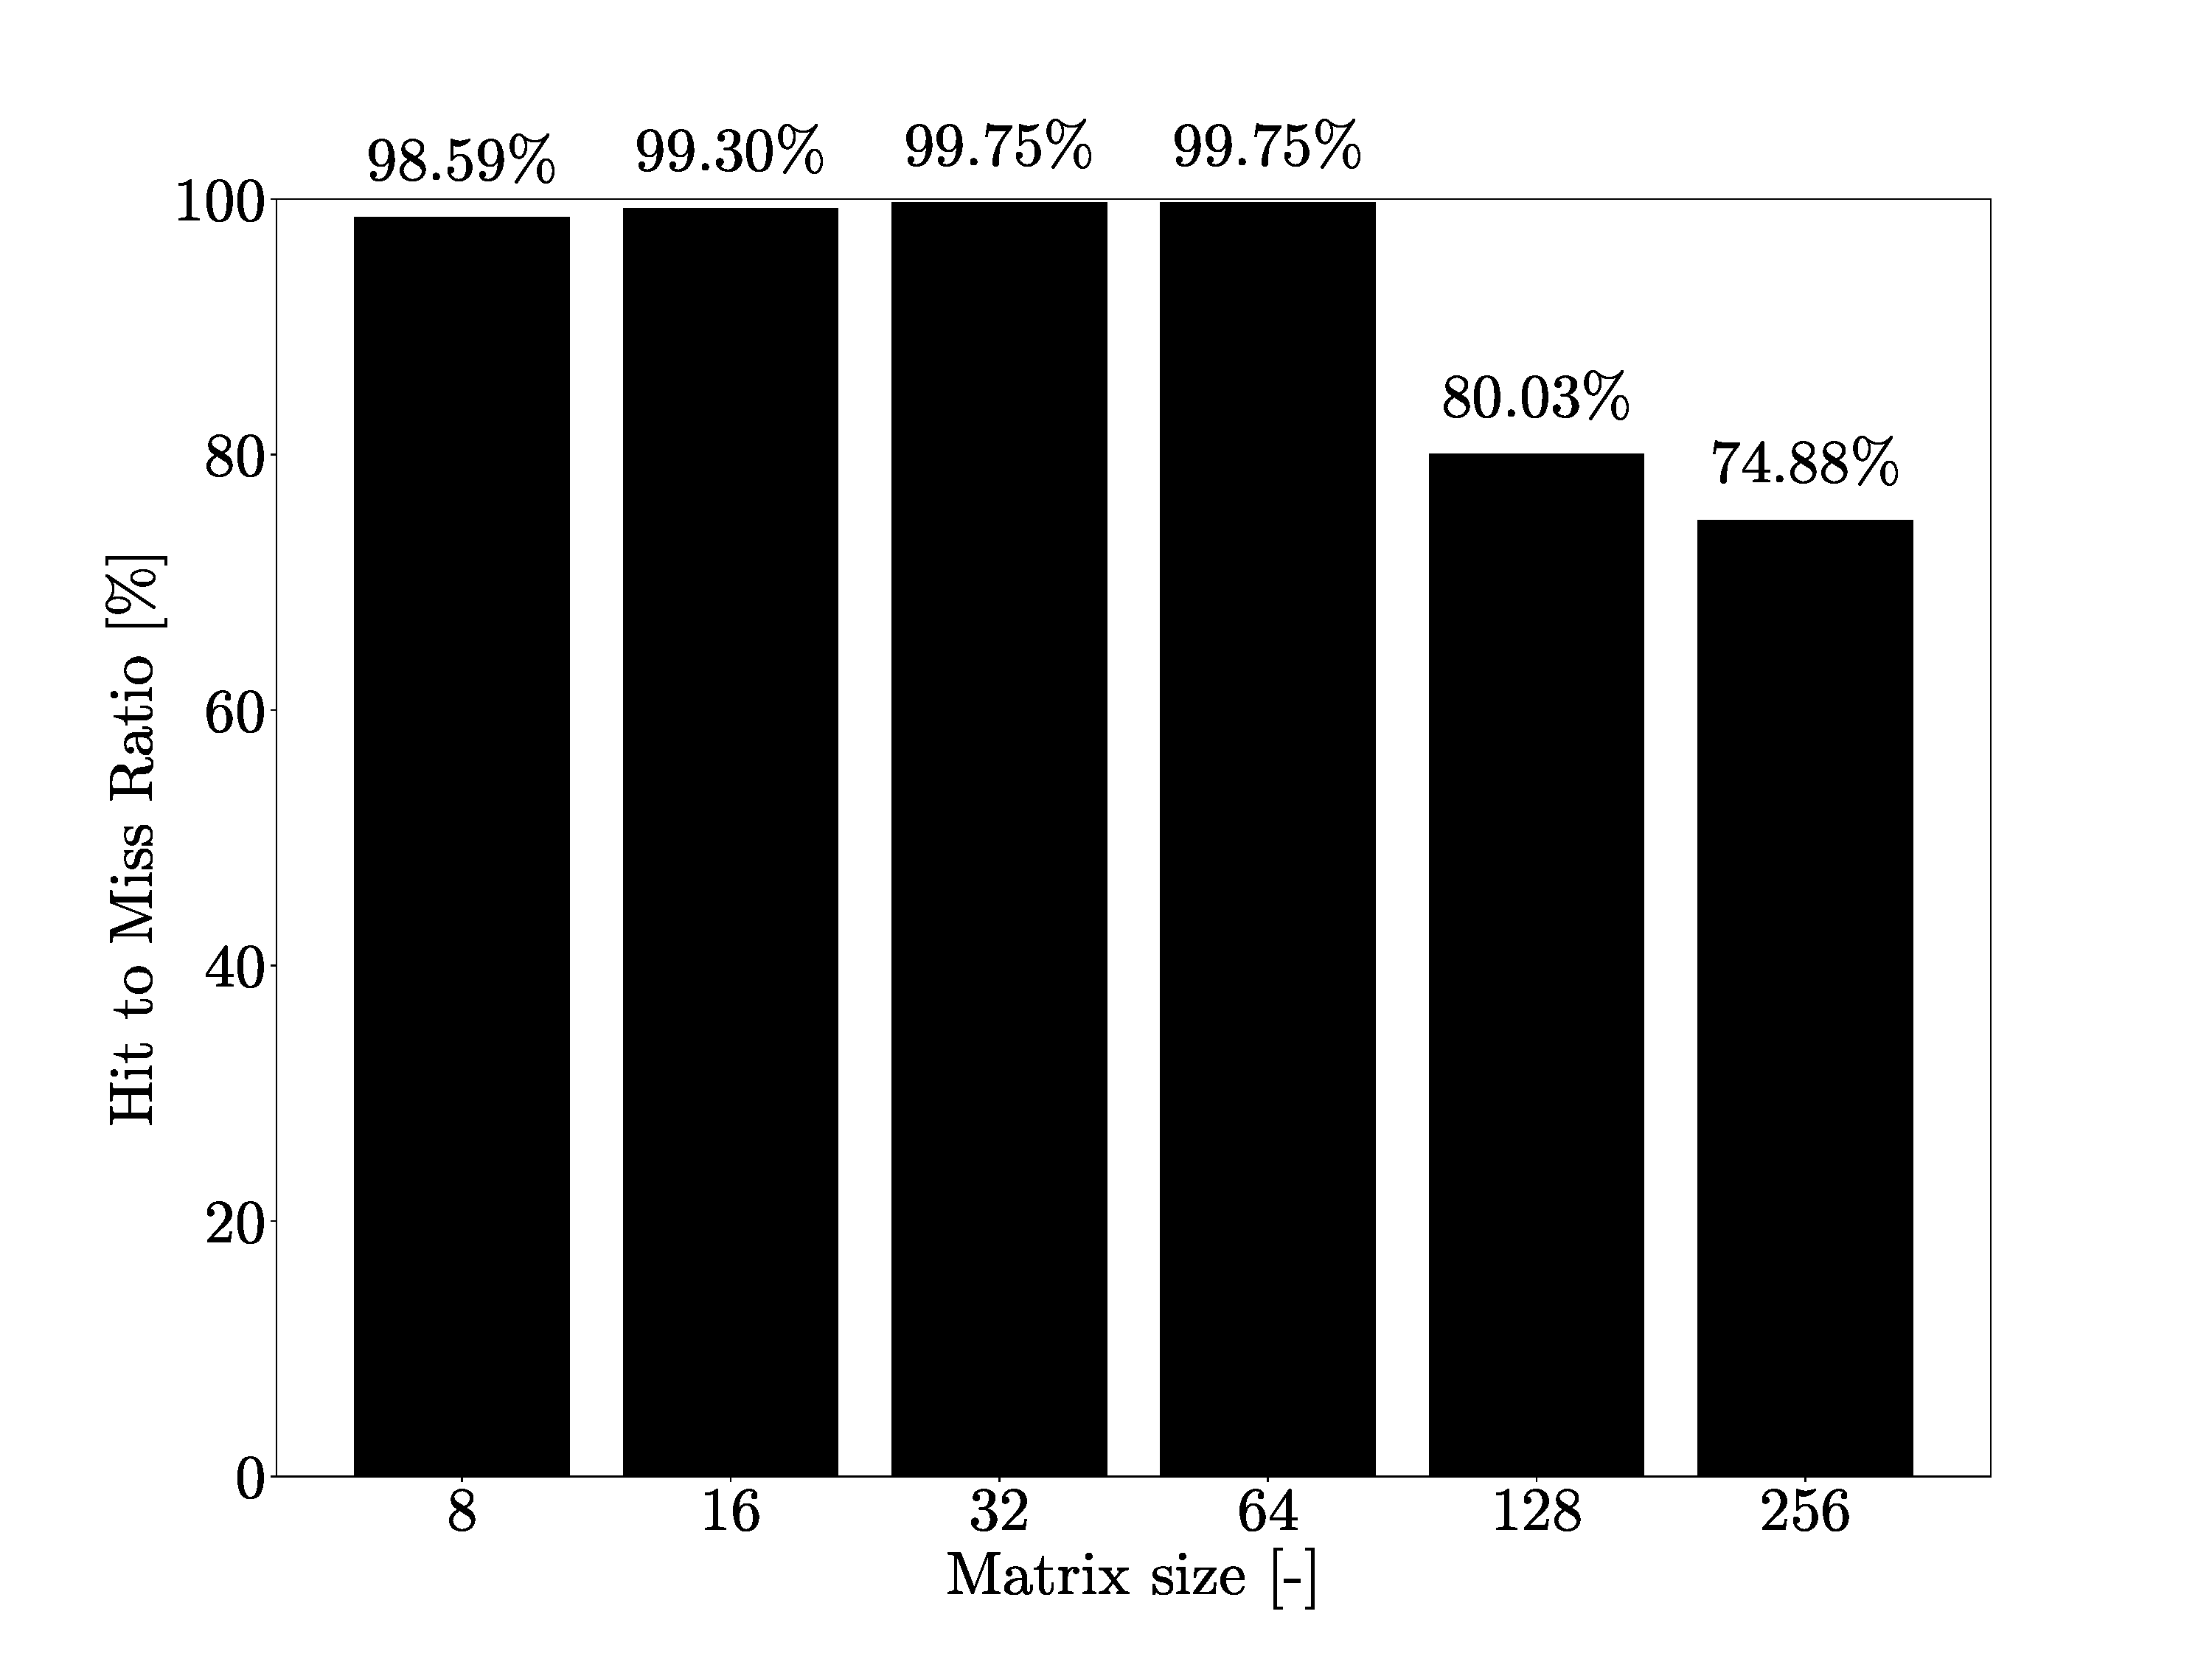
\includegraphics[width=0.75\textwidth]{figures/05-analysis/mm_naive_results.pdf}
	\captionof{figure}{HMR visualization for the naive matrix multiplication algorithm}
	\label{fig:mm_naive_results}
\end{center}

\noindent The cache-optimized block-based approach, detailed in Tables (\ref{tab:performance_metrics_16}) to (\ref{tab:performance_metrics_256}), demonstrates significantly
improved cache utilization. By dividing the matrices into smaller blocks, this method enhances data locality and reduces cache misses, particularly for larger matrices. The block
size plays a critical role in optimizing cache performance, as reflected in the varying hit rates. For instance, with a matrix size of \( 128^2 \), a block size of 32 achieves the
highest hit rate of 99.71\%, substantially better than the naive approach.

\begin{figure}[!htbp]
    \centering
    \begin{subfigure}{0.5\textwidth}
      \centering
      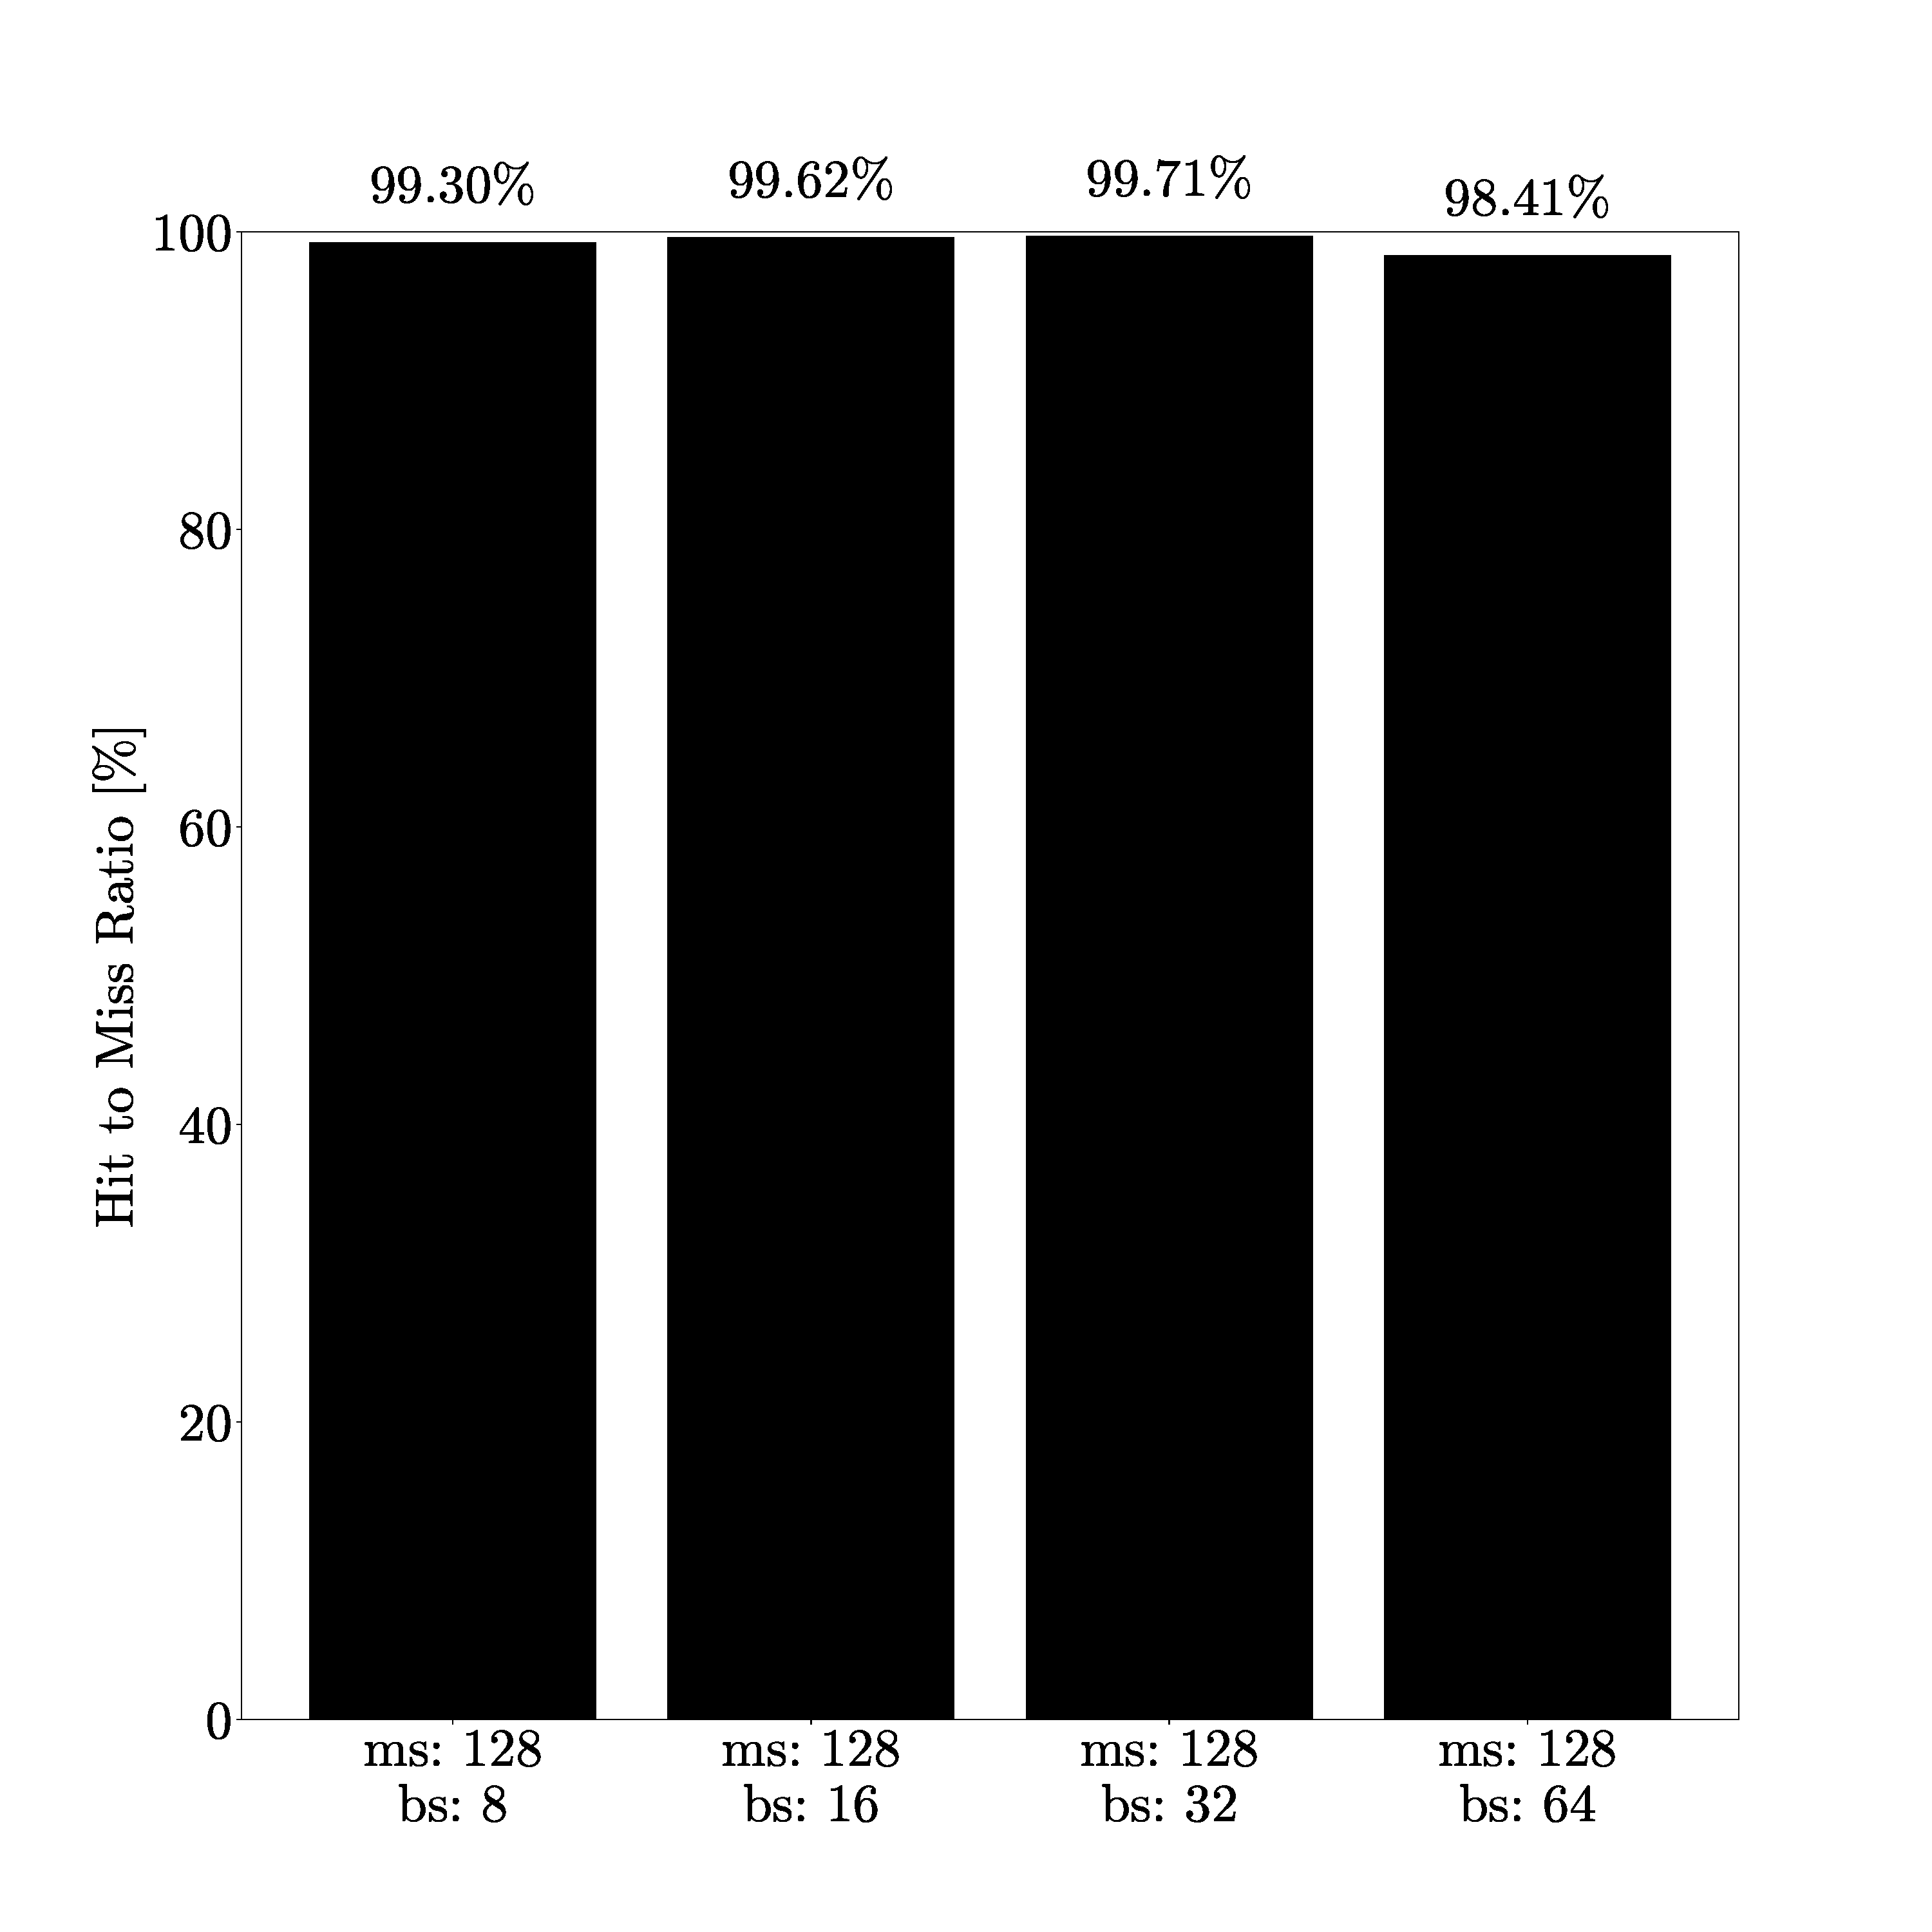
\includegraphics[width=1\linewidth]{figures/05-analysis/block_ms128.pdf}
    \end{subfigure}%
    \begin{subfigure}{0.5\textwidth}
      \centering
      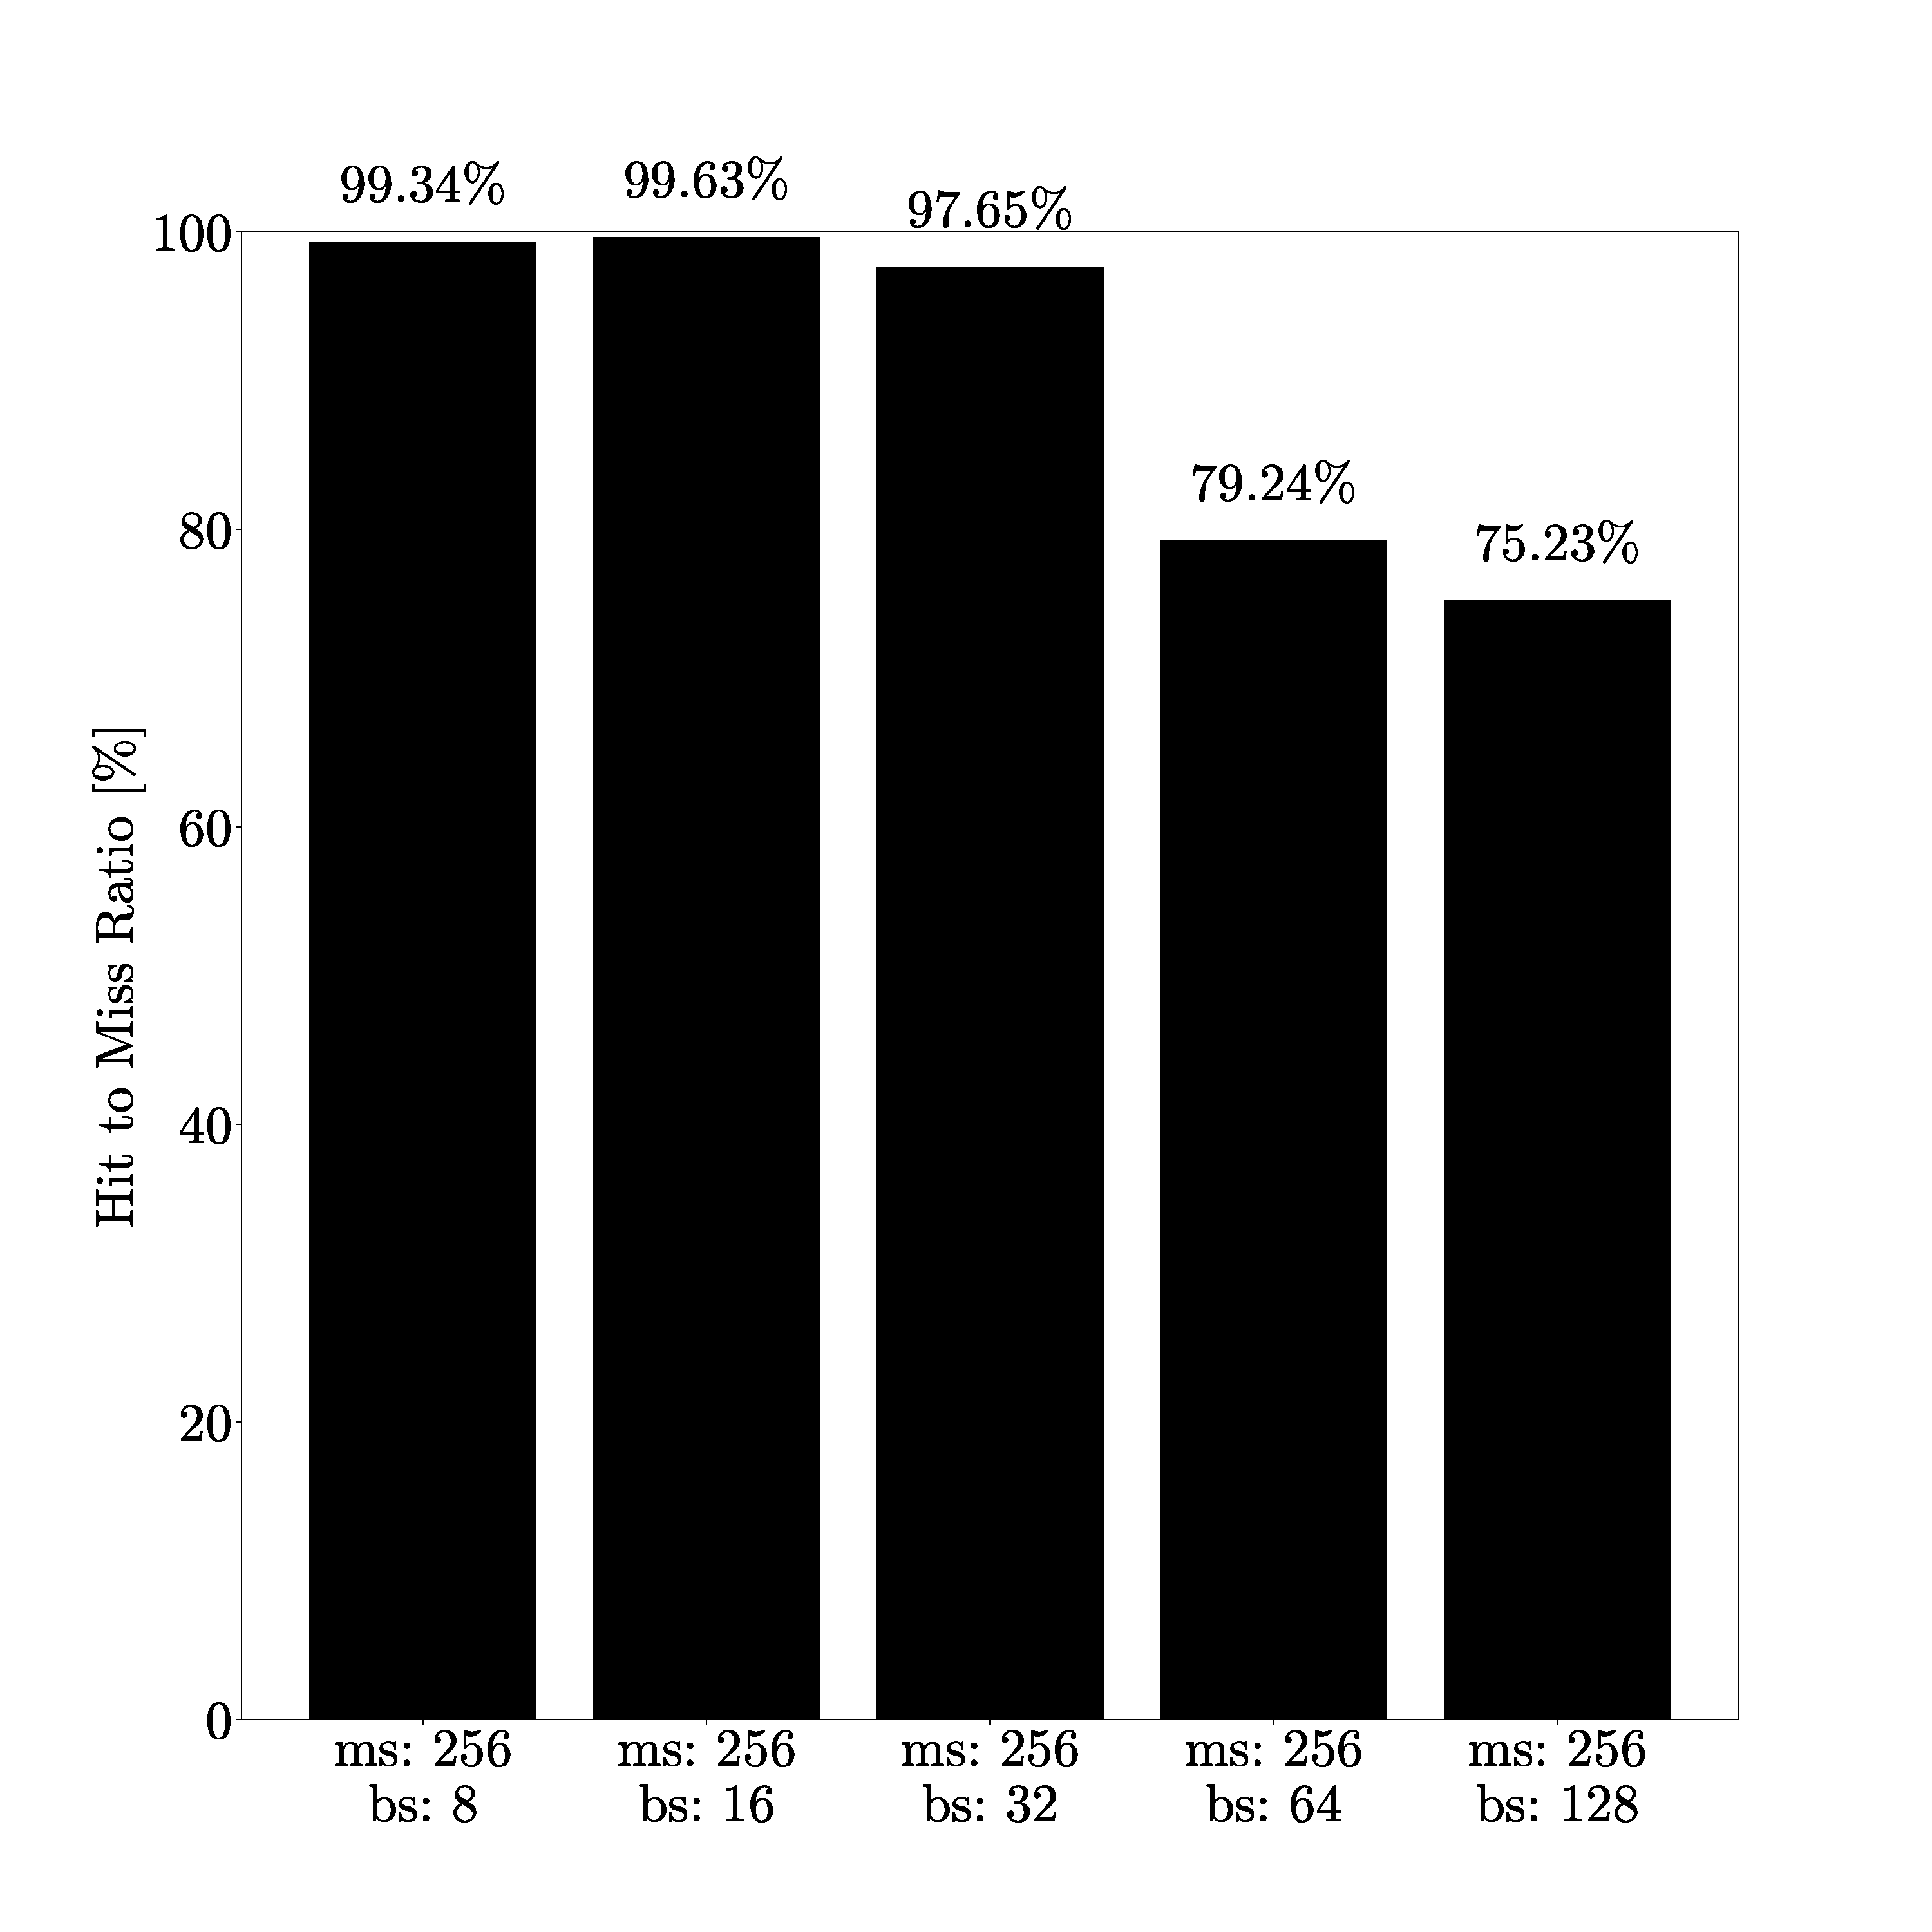
\includegraphics[width=1\linewidth]{figures/05-analysis/block_ms256.pdf}
    \end{subfigure}
    \caption{HMR visualization for a block-based algorithm for matrices of sizes 128 and 256 with various block sizes}
\end{figure}

\noindent It is important to note that decreasing block size has caused an increase in the total instructions executed. For example, the naive approach for matrix size \( 256^2 \) required
174,620,452 instructions, while the block-based approach with block size of 32 required 277,988,449 instructions - a 59\% increase. Overall, the amount of instructions executed
increases as the block size decreases, with block sizes of 8, 32, and 128 requiring 288,790,285 (65.4\% increase), 277,988,449 (59.2\% increase), and 275,419,880 (57.7\% increase)
instructions, respectively.

